% Version 1.2 of SN LaTeX, November 2022
%
% See section 11 of the User Manual for version history 
%
%%%%%%%%%%%%%%%%%%%%%%%%%%%%%%%%%%%%%%%%%%%%%%%%%%%%%%%%%%%%%%%%%%%%%%
%%                                                                 %%
%% Please do not use \input{...} to include other tex files.       %%
%% Submit your LaTeX manuscript as one .tex document.              %%
%%                                                                 %%
%% All additional figures and files should be attached             %%
%% separately and not embedded in the \TeX\ document itself.       %%
%%                                                                 %%
%%%%%%%%%%%%%%%%%%%%%%%%%%%%%%%%%%%%%%%%%%%%%%%%%%%%%%%%%%%%%%%%%%%%%

%%\documentclass[referee,sn-basic]{sn-jnl}% referee option is meant for double line spacing

%%=======================================================%%
%% to print line numbers in the margin use lineno option %%
%%=======================================================%%

%%\documentclass[lineno,sn-basic]{sn-jnl}% Basic Springer Nature Reference Style/Chemistry Reference Style

%%======================================================%%
%% to compile with pdflatex/xelatex use pdflatex option %%
%%======================================================%%

%%\documentclass[pdflatex,sn-basic]{sn-jnl}% Basic Springer Nature Reference Style/Chemistry Reference Style


%%Note: the following reference styles support Namedate and Numbered referencing. By default the style follows the most common style. To switch between the options you can add or remove “Numbered” in the optional parenthesis. 
%%The option is available for: sn-basic.bst, sn-vancouver.bst, sn-chicago.bst, sn-mathphys.bst. %  
 
%%\documentclass[sn-nature]{sn-jnl}% Style for submissions to Nature Portfolio journals
%%\documentclass[sn-basic]{sn-jnl}% Basic Springer Nature Reference Style/Chemistry Reference Style
\documentclass[sn-mathphys,Numbered]{sn-jnl}% Math and Physical Sciences Reference Style
%%\documentclass[sn-aps]{sn-jnl}% American Physical Society (APS) Reference Style
%%\documentclass[sn-vancouver,Numbered]{sn-jnl}% Vancouver Reference Style
%%\documentclass[sn-apa]{sn-jnl}% APA Reference Style 
%%\documentclass[sn-chicago]{sn-jnl}% Chicago-based Humanities Reference Style
%%\documentclass[default]{sn-jnl}% Default
%%\documentclass[default,iicol]{sn-jnl}% Default with double column layout

%%%% Standard Packages
%%<additional latex packages if required can be included here>

\usepackage{graphicx}%
\usepackage{multirow}%
\usepackage{amsmath,amssymb,amsfonts}%
\usepackage{amsthm}%
\usepackage{mathrsfs}%
\usepackage[title]{appendix}%
\usepackage{xcolor}%
\usepackage{textcomp}%
\usepackage{manyfoot}%
\usepackage{booktabs}%
\usepackage{algorithm}%
\usepackage{algorithmicx}%
\usepackage{algpseudocode}%
\usepackage{listings}%
%%%%

%%%%%=============================================================================%%%%
%%%%  Remarks: This template is provided to aid authors with the preparation
%%%%  of original research articles intended for submission to journals published 
%%%%  by Springer Nature. The guidance has been prepared in partnership with 
%%%%  production teams to conform to Springer Nature technical requirements. 
%%%%  Editorial and presentation requirements differ among journal portfolios and 
%%%%  research disciplines. You may find sections in this template are irrelevant 
%%%%  to your work and are empowered to omit any such section if allowed by the 
%%%%  journal you intend to submit to. The submission guidelines and policies 
%%%%  of the journal take precedence. A detailed User Manual is available in the 
%%%%  template package for technical guidance.
%%%%%=============================================================================%%%%

%\jyear{2021}%

%% as per the requirement new theorem styles can be included as shown below
\theoremstyle{thmstyleone}%
\newtheorem{theorem}{Theorem}%  meant for continuous numbers
%%\newtheorem{theorem}{Theorem}[section]% meant for sectionwise numbers
%% optional argument [theorem] produces theorem numbering sequence instead of independent numbers for Proposition
\newtheorem{proposition}[theorem]{Proposition}% 
%%\newtheorem{proposition}{Proposition}% to get separate numbers for theorem and proposition etc.

\theoremstyle{thmstyletwo}%
\newtheorem{example}{Example}%
\newtheorem{remark}{Remark}%

\theoremstyle{thmstylethree}%
\newtheorem{definition}{Definition}%

\raggedbottom
%%\unnumbered% uncomment this for unnumbered level heads

\begin{document}

\title{Exploring the Relationship between Review Star Rating and Text Sentiment: Insights from an Ordered Probit Approach}

\subtitle{22203640}

%%=============================================================%%
%% Prefix	-> \pfx{Dr}
%% GivenName	-> \fnm{Joergen W.}
%% Particle	-> \spfx{van der} -> surname prefix
%% FamilyName	-> \sur{Ploeg}
%% Suffix	-> \sfx{IV}
%% NatureName	-> \tanm{Poet Laureate} -> Title after name
%% Degrees	-> \dgr{MSc, PhD}
%% \author*[1,2]{\pfx{Dr} \fnm{Joergen W.} \spfx{van der} \sur{Ploeg} \sfx{IV} \tanm{Poet Laureate} 
%%                 \dgr{MSc, PhD}}\email{iauthor@gmail.com}
%%=============================================================%%

\author{\fnm{Alexandros} \sur{Doganis}}

\affil{\orgdiv{COMP0047 Data Science}, \orgname{UCL}}

%%==================================%%
%% sample for unstructured abstract %%
%%==================================%%

% \abstract{The abstract serves both as a general introduction to the topic and as a brief, non-technical summary of the main results and their implications. Authors are advised to check the author instructions for the journal they are submitting to for word limits and if structural elements like subheadings, citations, or equations are permitted.}

%%================================%%
%% Sample for structured abstract %%
%%================================%%

% \abstract{\textbf{Purpose:} The abstract serves both as a general introduction to the topic and as a brief, non-technical summary of the main results and their implications. The abstract must not include subheadings (unless expressly permitted in the journal's Instructions to Authors), equations or citations. As a guide the abstract should not exceed 200 words. Most journals do not set a hard limit however authors are advised to check the author instructions for the journal they are submitting to.
% 
% \textbf{Methods:} The abstract serves both as a general introduction to the topic and as a brief, non-technical summary of the main results and their implications. The abstract must not include subheadings (unless expressly permitted in the journal's Instructions to Authors), equations or citations. As a guide the abstract should not exceed 200 words. Most journals do not set a hard limit however authors are advised to check the author instructions for the journal they are submitting to.
% 
% \textbf{Results:} The abstract serves both as a general introduction to the topic and as a brief, non-technical summary of the main results and their implications. The abstract must not include subheadings (unless expressly permitted in the journal's Instructions to Authors), equations or citations. As a guide the abstract should not exceed 200 words. Most journals do not set a hard limit however authors are advised to check the author instructions for the journal they are submitting to.
% 
% \textbf{Conclusion:} The abstract serves both as a general introduction to the topic and as a brief, non-technical summary of the main results and their implications. The abstract must not include subheadings (unless expressly permitted in the journal's Instructions to Authors), equations or citations. As a guide the abstract should not exceed 200 words. Most journals do not set a hard limit however authors are advised to check the author instructions for the journal they are submitting to.}

% \keywords{keyword1, Keyword2, Keyword3, Keyword4}

%%\pacs[JEL Classification]{D8, H51}

%%\pacs[MSC Classification]{35A01, 65L10, 65L12, 65L20, 65L70}

\maketitle
\tableofcontents

\section{Introduction}\label{sec1}

While it is widely understood that review ratings in most domains tend to be polarized to the extremes following a J-curve distribution \cite{hu2006can}, we sought to explore how this phenomenon relates to the sentiment of accompanying review text and ultimately determine how strongly the sentiment of review text relates to its accompanying star rating. We hypothesized that this would be a strong relationship given that a review's rating and text are respectively quantitative and qualitative representations measuring the same experience.

\section{Methodology}\label{sec2}

\subsection{Data}
We analyzed the Yelp Dataset of business reviews \cite{yelpdataset}. To eliminate cultural bias, data was localized to reviews left on businesses within California. In preparation for sentiment analysis, the data was cleaned such that only non-empty, English reviews were considered.

\subsection{Sentiment Analysis}
In order to determine a text's sentiment, we used the  Valence Aware Dictionary and sEntiment Reasoner (VADER) \cite{hutto2014vader}, a rule-based sentiment analysis tool pre-trained on social media data. These rules are derived from its scored lexicon containing not only words, but emoticons, emojis, colloquialisms, and unconventional punctuations, each with a a pre-assigned sentiment value; this approach attempts to capture linguistic nuances more directly than probabilistic or Deep-Learning based approaches.

Using VADER, each review $i$ was assigned a sentiment score comprised of the probability that the text is positive, negative, or neutral such that:
\begin{equation}\label{prob_sum}
    P_{pos}(i) + P_{neg}(i) + P_{neu}(i) = 1
\end{equation}

thus completing our feature selection.

\subsection{Statistical Analysis}
\subsubsection{Visualization}
Visualization of the distribution of text sentiment for each star rating (see Fig. \ref{fig:sent_plot}) was achieved by plotting the polarity against the neutrality for every sample point such that:
\begin{equation}\label{polarity}
    Polarity(i) = P_{pos}(i) - P_{neg}(i)
\end{equation}
To distinguish distributions, each point was color coded and alpha layered according to its star rating \cite{matlab}. The mean of each distribution was additionally overlaid on the plot to aid in visual trend identification.

\subsubsection{Correlation Matrix}

In order to more formally assess the strength of our hypothesis, we computed a correlation matrix $R$ using Spearman's rank correlation coefficient $\rho_s$ \cite{seabold2010statsmodels}, given by:

\begin{equation}
\rho_s(A, B) = 1 - \frac{6 \sum_{i=1}^{n} d_i^2}{n(n^2 - 1)}
\end{equation}
\begin{equation}
R =
\begin{bmatrix}
1 & \rho_s(A, B) \\
\rho_s(B, A) & 1
\end{bmatrix}
\end{equation}

where $d_i$ is the difference between the ranks of corresponding variables $A$ and $B$ for each observation $i$, and $n$ is the number of observations \cite{fisher1958statistical}.

Spearman's rank correlation coefficient was chosen over the more straightforward Pearson's correlation coefficient as Pearson's is only able to measure linear relationships between variables, while Spearman's adaptation of Pearson can capture the monotonic relationship present between our variables. Given that star rating is a categorical variable (integers 1 - 5), Spearman's was more suitable and likely to result in reliable insights.


\subsubsection{Classification}
Following from our initial analysis and building on the trends identified, we sought to construct a classification model using our sentiment scores to predict star rating; the performance and component parameters of such a model can be harnessed to definitively assess the strength of the relationship.

Our dependant star rating variable is not only categorical, but ordinal i.e., has a natural order. Following from this, we utilized an ordered probit model \cite{seabold2010statsmodels}, which is specifically designed to capture the cumulative probability for each ordinal category; this is in contrast to linear or multinomial logistic regression models not intended to capture ordinal relationships.

Such a model functions by identifying a vector of parameters $\boldsymbol{\beta}$ from which we can identify the predictive power of each feature, such that:

\begin{equation}
    y^* = \boldsymbol{\beta} \textbf{x}^T - \epsilon
\end{equation}

where $y^*$ is an underlying, un-observable dependant variable (overarching rating in our case), $\textbf{x}$ is a vector of independent variables (our sentiment scores), and $\epsilon$ is an error term \cite{greene2012econometric}.

Given that the un-observable $y^*$ is in reality our ordered star rating categories 1 to 5, we can define these observable categories, $y$, via a series of thresholds $\mu_i$ such that:

\begin{equation}
    y =
    \begin{cases}
        1 & \text{if }     y^* \leq \mu_0, \\
        2 & \text{if } \mu_0 < y^* \leq \mu_1, \\
        3 & \text{if } \mu_1 < y^* \leq \mu_2, \\
        4 & \text{if } \mu_2 < y^* \leq \mu_3, \\
        5 & \text{if } \mu_3 < y^*
    \end{cases}
\end{equation}

Next we estimated $\beta$ for each feature in our feature vector $\textbf{x}$ and $\mu_i$ for each categorical threshold. As identified in Eq. \ref{prob_sum}, any one sentiment probability can be calculated given the other two, thus making inclusion of all three features in our model redundant; we considered only positive and negative scores. To make this estimation, we used Maximum Likelihood Estimation (MLE) to maximize the likelihood function $L$ representing the joint probability of the observed data given the model, given by:

\begin{equation}
L(\boldsymbol{\beta}, \boldsymbol{\mu} | \textbf{x}, \textbf{y}) = \prod_{i=1}^n P(y_i | \textbf{x}_i, \boldsymbol{\beta}, \boldsymbol{\mu})
\end{equation}

where $n$ is the number of observations, and $P(y_i | \textbf{x}_i, \boldsymbol{\beta}, \boldsymbol{\mu})$ is the probability of observing a star rating $y_i$ given the independent positive and negative sentiment score variables $\textbf{x}_i$ and their corresponding parameters $\beta$ and $\mu$.

Upon completion of the MLE, we calculated their test statistic ($z$-value) given by:

\begin{equation}
z_i = \frac{\hat{\beta}_i}{SE(\hat{\beta}_i)}
\end{equation}

where $\hat{\beta}_i$ is the estimated coefficient for the $i$-th variable and $SE(\hat{\beta}_i)$ is the standard error of the estimated coefficient. 

We then determined the significance of the estimated coefficients by computing the p-value of each using the cumulative distribution function of the standard normal distribution, $\Phi(z)$, and calculating the probability that a random variable from $\Phi(z)$ would be less than or equal to $z$, given by:
\begin{equation}
p_i = 2 \times (1 - \Phi(|z_i|))
\end{equation}

\textbf{Note:} As our star ratings distribution followed a J-curve, we under-sampled the data to ensure each distribution was inline with the least common star rating (2 stars) in order to avoid over-fitting the data and to increase the model's predictive power.\\

The model's performance was evaluated using the precision, recall, and F1 score for each star rating, as well the model's overall accuracy and weighted F1 score, respectively given by:

\begin{equation}
\text{Precision} = \frac{\text{True Positives}}{\text{True Positives} + \text{False Positives}}
\end{equation}

\begin{equation}
\text{Recall} = \frac{\text{True Positives}}{\text{True Positives} + \text{False Negatives}}
\end{equation}

\begin{equation}
\text{F1} = 2 \cdot \frac{\text{Precision} \times \text{Recall}}{\text{Precision} + \text{Recall}}
\end{equation}

\begin{equation}
\text{Accuracy} = \frac{\text{True Positives} + \text{True Negatives}}{\text{Total Observations}}
\end{equation}

\begin{equation} \label{eq:weighted_f1}
\text{Weighted F1} = \frac{1}{\sum_{i=1}^5 w_i} \sum_{i=1}^5 w_i \cdot \text{F1}_i
\end{equation}

where $w_i$ is the weight for the star rating $i$ proportionate to its representation in the dataset, and $\text{F1}_i$ is the F1 score for the star rating $i$.

\section{Results}\label{sec3}

\subsection{Visualization}
\begin{figure}[h!]
    \centering
    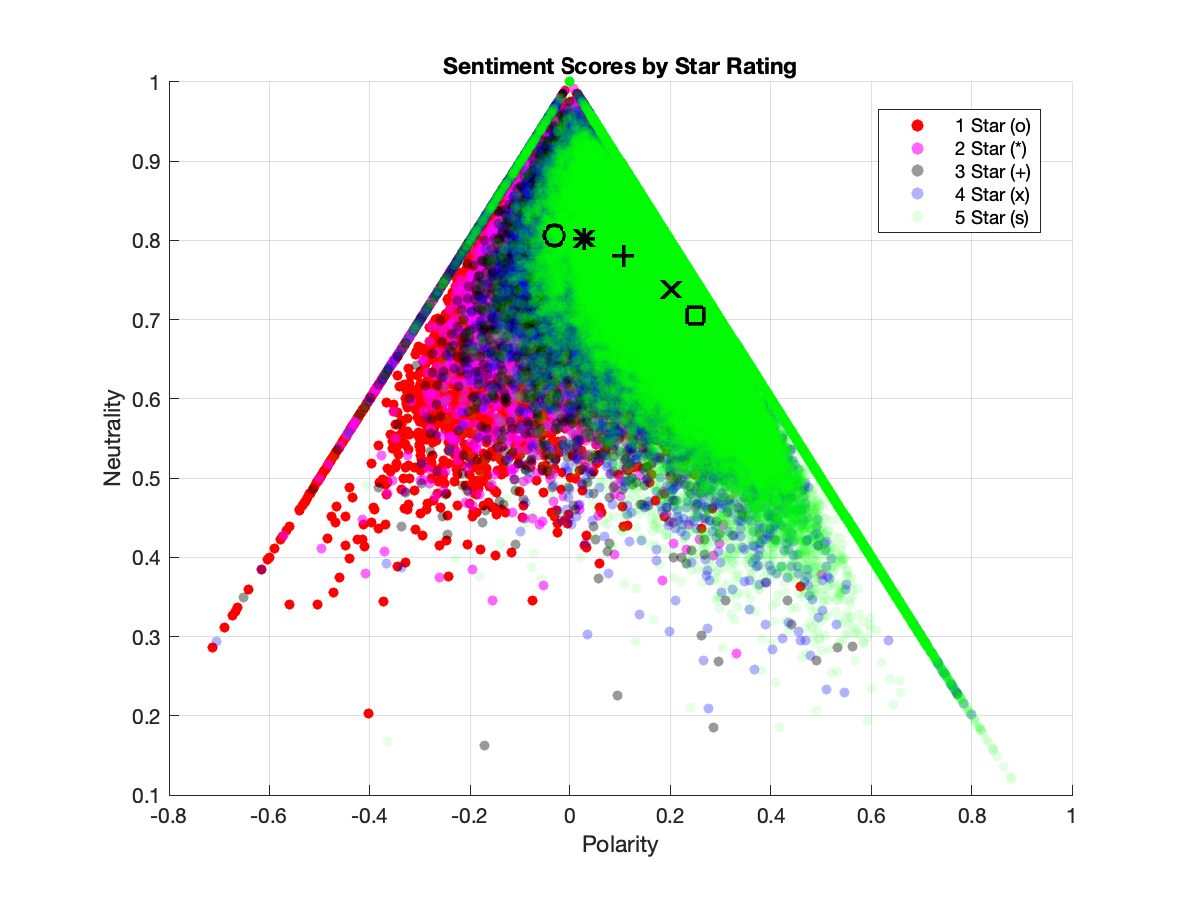
\includegraphics[width=\linewidth]{sent_scores_by_rating.eps}
    \caption{Polarity vs Neutrality, grouped by star rating. The parenthetical beside each star rating in the legend denotes the symbol marking the mean of the respective distribution. Note that the samples are triangularly bounded due to their relationship (see Eq. \ref{prob_sum}).}
    \label{fig:sent_plot}
\end{figure}

Fig. \ref{fig:sent_plot} visually identifies that the means of each star rating's sentiment distributions become more positive and less neutral as star rating increases and vice versa, inline with our hypothesis. This effect becomes more pronounced the higher the star rating.

\subsection{Correlation Matrix}
\begin{table}[h!]
\centering
\begin{tabular}{l|cccc}
           & stars     & neg       & neu       & pos       \\ \hline
stars & 1.00 & -0.50 & -0.38 & 0.58 \\
neg & -0.50 & 1.00 & 0.17 & -0.55 \\
neu & -0.38 & 0.17 & 1.00 & -0.88 \\
pos & 0.58 & -0.55 & -0.88 & 1.00 \\
\end{tabular}
\caption{Spearman's Correlation Matrix}
\label{tab:spearman_correlation}
\end{table}

Table \ref{tab:spearman_correlation} shows moderately positive correlation (0.58) between positive sentiment and high star rating. Similarly, it shows moderately negative correlation (-0.50) between negative sentiment and high star rating. Neutral sentiment also shows a slight negative correlation (-0.38) to high star rating. 

\subsection{Classification}

\begin{table}[h!]
\centering
\begin{tabular}{l|c|c|c|c|c|c}
\hline
Dep. Variable & Log-Likelihood & AIC & BIC & No. Observations & Df Residuals & Df Model \\ \hline
stars         & -1.6000e+05     & 3.200e+05 & 3.201e+05 & 122,131         & 122,125      & 6       \\ \toprule
\end{tabular}
\begin{tabular}{l|c|c|c|c|c|c}
\hline
& coef   & std err & z        & P$>$$|$z$|$ & [0.025 & 0.975] \\ \hline
neg & -7.26 & 0.062 & -117.308 & 0.000 & -7.38 & -7.14 \\
pos & 6.12 & 0.035 & 174.264 & 0.000 & 6.06 & 6.19 \\ \midrule
$\mu_0$ & -0.639 & 0.009 \\
$\mu_1$ & -0.212 & 0.006 \\
$\mu_2$ & -0.117 & 0.005 \\
$\mu_3$ & -0.215 & 0.006 \\ \botrule
\end{tabular}
\caption{Ordered model results star rating classification on sentiment scores. Note that $\boldsymbol{\mu}$ are ancillary variables and therefore do not carry testable significance}
\label{tab:ordered_model_results}
\end{table}

Table \ref{tab:ordered_model_results} shows the estimated $\boldsymbol{\beta}$ coefficients. Both positive and negative sentiment scores carry highly positive (6.12) and highly negative (-7.26) coefficients, respectively. Both $\beta$ values carry p-values $< 0.05$, indicating that these values are significant and that we can reject the null hypothesis that sentiment scores and star ratings have no relationship.

The $\boldsymbol{\mu}$ threshold values also shown in Table \ref{tab:ordered_model_results} show that the distance between rating categories follows an ordinal structure between the first four categories, with each being larger than the next, with the exception of $\mu_3$ (4/5).

\begin{table}[h!]
\centering
\begin{tabular}{l|c|c|c}
\hline
            & Precision & Recall & F1 Score \\ \hline
Star Rating 1 & 0.532     & 0.581  & 0.555    \\
Star Rating 2 & 0.341     & 0.155  & 0.214    \\
Star Rating 3 & 0.331     & 0.602  & 0.427    \\
Star Rating 4 & 0.350     & 0.121  & 0.180    \\
Star Rating 5 & 0.495     & 0.541  & 0.517    \\ \hline
\end{tabular}

\begin{tabular}{c|c}
Overall Accuracy: & 0.409 \\
Weighted F1 Score: & 0.381
\end{tabular} \botrule
\caption{Ordered model performance metrics for each star rating.}
\label{tab:performance_metrics}
\end{table}

Table \ref{tab:performance_metrics} indicates that the model can correctly predict star rating based on sentiment scores with 40.9\% accuracy. The model has the highest precision ($\approx0.5$) at the extreme star ratings and is less precise ($\approx0.3$) in the middling ratings. Similarly, the model has high recall ($\approx0.5$) at the extremes, however has the highest recall ($\approx0.6$) at a star rating of 3, with star ratings 2 and 4 having quite low recall ($\approx0.1$). The model's weighted F1 score (see Eq. \ref{eq:weighted_f1}) is a low 38.1\%.


\section{Conclusion}\label{sec4}

Both the plot in Fig. \ref{fig:sent_plot} and the correlation values shown in Table \ref{tab:spearman_correlation} indicate that as ratings increase, sentiment becomes strictly more positive. In addition, the strong negative correlation between positive and neutral sentiment indicates that neutrality decreases with an increase in star rating inline with the trend identified in Fig. \ref{fig:sent_plot}. When combined with the similar high positive and negative $\beta$ coefficients in \ref{tab:ordered_model_results}, these results collectively support our initial hypothesis of a strong relationship between review text sentiment and star rating.

Despite this, the ordered probit model did not perform well; the inconsistency in the categories' ordinal relationship in conjunction with the model's low accuracy and weighted F1 score suggest that it is generally a poor classifier. A notable exception, the model was better at predicting extreme values which follows given that these categories were the least bounded, each having only one $\mu$ threshold bound. Ultimately, the performance of this classifier suggests that while there is indeed a relationship between the review text sentiment and star rating, it may not be a strong and simple one; the intra-correlations between sentiment scores and distances between ordinal thresholds indicate that their relationship is rich with nuance.

This analysis has so far considered VADER to be a trustworthy ground-truth for sentiment classification, however the study might be  improved through involvement of a more sophisticated or purpose-built sentiment classifier; this classifier might consider additional factors such as context, sarcasm, or idiomatic expressions, or may learn sentimental relationships completely independently, each of these possibly providing a more accurate representation of sentiment.

Additionally, it is essential to acknowledge that star ratings are subjective and can vary significantly between individuals, making them an inherently imprecise measure. This subjectivity may contribute to our poor ordinal relationship in Table \ref{tab:ordered_model_results} the difficulty in accurately predicting star ratings based solely on sentiment scores without the inclusion of exogenous data. A potentially more accurate measure of a business's performance could be the average star rating across all reviews, which would smooth out individual variations and provide a more representative view of overall customer sentiment. Future research could investigate the relationship between average star ratings and aggregated sentiment scores, potentially providing more reliable and actionable insights for businesses seeking to understand and improve their customer experience.


%%=============================================%%
%% For submissions to Nature Portfolio Journals %%
%% please use the heading ``Extended Data''.   %%
%%=============================================%%

%%=============================================================%%
%% Sample for another appendix section			       %%
%%=============================================================%%

%% \section{Example of another appendix section}\label{secA2}%
%% Appendices may be used for helpful, supporting or essential material that would otherwise 
%% clutter, break up or be distracting to the text. Appendices can consist of sections, figures, 
%% tables and equations etc.


%%===========================================================================================%%
%% If you are submitting to one of the Nature Portfolio journals, using the eJP submission   %%
%% system, please include the references within the manuscript file itself. You may do this  %%
%% by copying the reference list from your .bbl file, paste it into the main manuscript .tex %%
%% file, and delete the associated \verb+\bibliography+ commands.                            %%
%%===========================================================================================%%

\bibliography{sn-bibliography}% common bib file
%% if required, the content of .bbl file can be included here once bbl is generated
%%\input sn-article.bbl


\end{document}
